\title{Operating Systems–2: CS3523 2019\\
Programming Assignment 5: \\
Implement Dining Philosopher’s using Conditional
Variables\\
Report}
\author{Sai Harsha Kottapalli\\CS17BTECH11036}
\date{April 9, 2019}

\documentclass[12pt]{article}
\usepackage{graphicx}
\usepackage[most]{tcolorbox}

\definecolor{bg}{RGB}{220,220,220}

\begin{document}
\maketitle

\section{Aim}
We have to solve the Dining Philosopher’s problem using conditional variables.\\
We then compare the average and worst-case time taken for each thread to access the critical section (shared resources) for different number of threads.

\section{Design \& implementation of the Program:}
We use conditional variables and a mutex to implement the Dining philosophers using monitor approach.
\subsection{Design}
\begin{enumerate}
\item Class \textbf{Dphil} acts as the the monitor in the c++ program.\\
	\begin{itemize}
	\item we define THINKING, HUNGRY, EATING states accessible by each philosopher.
	\item A list of conditional variables, one for each philosopher.
	\item A mutex \textbf{monitor} for implementing monitor's mutual exclusion property(wrapped for every function inside the class).
	\item We initialise with all philosophers in THINKING mode, mutex monitor to be available.
	\item \textbf{test()} to check if a particular philosopher can eat at a given instance.
	\item Algorithm:\\
	\begin{tcolorbox}[enhanced jigsaw,colback=bg,boxrule=0pt,arc=0pt]
    void test(int i) \{\\
      $\hspace*{10mm}$if ((state[(i + (n$\textunderscore$p - 1)) \% n$\textunderscore$p] != 											EATING) \&\&\\
          $\hspace*{20mm}$ (state[i] == HUNGRY) \&\&\\
          $\hspace*{20mm}$ (state[(i + 1) \% n$\textunderscore$p] != EATING)) \{\\
        $\hspace*{20mm}$ state[i] = EATING;\\
        $\hspace*{20mm}$ pthread$\textunderscore$cond$\textunderscore$signal(\&self[i]);\\
      $\hspace*{10mm}$\}\\
      $\hspace*{10mm}$ return;\\
    \}\\
  	\end{tcolorbox}
	\item \textbf{pickup()} - calls test() to check if this philosopher can eat, else calls wait().\\
	Here, pthread$\textunderscore$cond$\textunderscore$wait() unlocks the mutex associated with it, before suspending this thread.\\
	When unlocked, the mutex is then locked.\\
	\item Algorithm:\\
	\begin{tcolorbox}[enhanced jigsaw,colback=bg,boxrule=0pt,arc=0pt]
    void putdown(int i) \{\\
      $\hspace*{10mm}$state[i] = HUNGRY;\\
      $\hspace*{10mm}$test(i);\\
      $\hspace*{10mm}$if (state[i] != EATING)\\
      $\hspace*{20mm}$  pthread$\textunderscore$cond$\textunderscore$wait(\&self[i], \&monitor);\\
      $\hspace*{10mm}$return;\\
    \}\\
  	\end{tcolorbox}
	\item \textbf{putdown()} - philosopher is done eating, puts down the chopstick(allows neighbours to pick this chopstick) and starts thinking.
	\item Algorithm:\\
	\begin{tcolorbox}[enhanced jigsaw,colback=bg,boxrule=0pt,arc=0pt]
    void putdown(int i) \{\\
      $\hspace*{10mm}$state[i] = THINKING;\\
      $\hspace*{10mm}$test((i + (n$\textunderscore$p - 1)) \% n$\textunderscore$p);\\
      $\hspace*{10mm}$test((i + 1) \% n$\textunderscore$p);\\
      $\hspace*{10mm}$return;\\
    \}\\
  	\end{tcolorbox}
  	\item We have to call functions in the following order:\\
 		\begin{tcolorbox}[enhanced jigsaw,colback=bg,boxrule=0pt,arc=0pt]
    	philosophers.pickup(id);\\
    	$\char`\\\char`\\$ EAT - CS\\
    	philosophers.putdown(id);\\
  	\end{tcolorbox}
	\end{itemize}
\end{enumerate}

\subsection{Critical Section :}
This part of the code should be accessed by atmost two non-consecutive philosophers respectively at a time.
\subsection{Entry Section :}
This part of the code is accessible for all the philosophers. The job of this code is to make sure atmost two non-consecutive philosophers are given access(allowed to take the corresponding chopsticks) to the critical section at a particular time.
\subsection{Exit Section :}
This part of the code is where the philosopher has executed the critical section(Ate) of the program, and will putdown his chopstick so that other philosopher can now enter the critical section(if any) while this philosopher completes the remainder section parallelly(Thinking).
\subsection{Average Waiting Time :}
This is defined as the amount of time each access to critical section takes after requesting for the same.
\subsection{Worst Waiting Time :}
This is defined as the highest amount of time taken by a philospher respectively to critical section takes after requesting for the same.
\subsection{getInput()}
This is a helper function which helps in keeping the code modular.\\
It reads the value of the following from the input file, specified in ReadMe.txt \\
\begin{itemize}
\item \textbf{Number of philosophers} - n
\item \textbf{Number of readers} - h\\
\item \textbf{lam1 and lam2}\\
Represents the mean of value of two exponential distribution curves which is to be constructed.\\
Given in milli-seconds.
\end{itemize}

\subsection{dining()}
The dining() function simulates a philosophers trying to get chopsticks to eat.\\
Only one phi at a time, can be inside the CS to avoid synchronization issues.

\subsection{currTime()}
Takes input time$\textunderscore$t structure to generate the time in HH:MM:SS syntax and return this as a string.

\subsection{Other important variables used}
\begin{itemize}
\item \textbf{exponential$\textunderscore$distribution}\\
Produces random non-negative floating-point values x, distributed according to probability density function defined for exponential distribution about the constant rate given as a parameter.
\item \textbf{default$\textunderscore$random$\textunderscore$engine}\\
This is a random number engine class that generates pseudo-random numbers.
\item \textbf{thread *th for writers and readers}\\
th$\textunderscore$w and th$\textunderscore$r are the pointers for storing the array of nw and nr threads respectively. This will be useful for later calling \textbf{join()} to properly exit the threads spawned previously.
\item \textbf{Average and worst waiting times for writers and readers}\\
Used to calculate the average time as well as worst waiting time, a writer/reader has to wait for getting access to the CS.\\
\end{itemize}

\section{Conditional Variables}
A condition(conditional variable) is a synchronization device which can be used to suspend threads until some condition is satisfied.\\
There is also a mutex associated with this conditional variable to avoid the race condition where a thread prepares to wait on a condition variable and another thread signals the condition just before the first thread actually waits on it.\\ 

\section{Output}
\begin{itemize}
\item Log file for dining philosophers.\\
This stores the events which occur throughout the simulation.\\
\\Example : \\
\textit{1st eat request by Thread 1 at 15:37:51}\\
\textit{1st eat request by Thread 4 at 15:37:51}\\
\textit{1st CS Entry by Philosopher Thread 4 at 15:37:51}\\
\textit{1st eat request by Thread 3 at 15:37:51}\\
\textit{1st eat request by Thread 2 at 15:37:51}\\
\textit{1st CS Exit by Philosopher Thread 4 at 15:37:51}\\
\item Times.txt\\
This file stores the average times as well as worst waiting time for philosophers.\\
The values are in milli-seconds.\\
\\Example: \\
\textit{Average waiting time for philosophers(ms): 0.804050}\\
\textit{Worst time taken for philosopher to eat(ms): 6.597000}\\
\end{itemize}

\newpage

\section{Comparision}
\subsection{Graphs}
\begin{figure}[ht!]
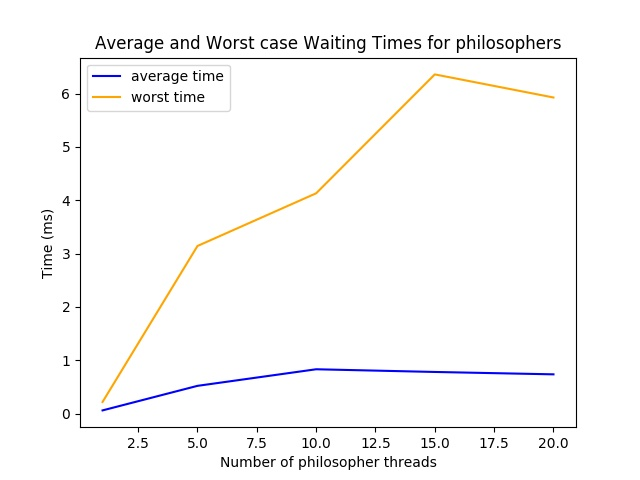
\includegraphics[width=150mm]{graph.jpg}
\caption{Average time taken and worst time taken to enter the CS by the philosophers}
\end{figure}

\newpage

\subsection{Notes}
\begin{itemize}
\item Parameters used for test cases:\\
n = 1, 5, 10, 15, 20\\
h = 10\\
$\Lambda _1$ = 1 milli-seconds and $\Lambda _2$ = 2 milli-seconds\\
\item Each of the plotted points is the average of 5 testcases.\\
\item We can infer that, as number of philosopher threads increases, the average value converges to some value.
\item As for worst case waiting time, though irregular, in general the worst case waiting time increases, as number of threads increases.
\item This is because, the given implementation has a drawback, that is starvation, hence the worst case waiting time will increase as number of philosophers increase.
\end{itemize}
\end{document}